\documentclass[12pt,a4paper]{article}

\usepackage[utf8]{inputenc}
\usepackage[T1]{fontenc}
\usepackage{graphicx}
\usepackage{hyperref}
\usepackage{geometry}
\usepackage{booktabs}
\usepackage{amssymb}
\usepackage{float}
\usepackage{enumitem}
\usepackage{fancyhdr}
\usepackage{xcolor}
\usepackage{listings}
\usepackage{tikz}
\usetikzlibrary{positioning, arrows.meta, shapes.geometric}
\usepackage{colortbl}
\usepackage{mdframed}
\usepackage{setspace}

\geometry{margin=1in, headheight=15pt}
\onehalfspacing

% Colors
\definecolor{primaryblue}{RGB}{26, 115, 232}
\definecolor{darkblue}{RGB}{13, 71, 161}
\definecolor{lightblue}{RGB}{232, 245, 253}
\definecolor{successgreen}{RGB}{46, 125, 50}
\definecolor{lightgray}{RGB}{248, 249, 250}

\hypersetup{colorlinks=true, linkcolor=darkblue, urlcolor=primaryblue}

% Code styling
\lstset{
    basicstyle=\ttfamily\small,
    breaklines=true,
    frame=single,
    backgroundcolor=\color{lightgray},
    numbers=left,
    numberstyle=\tiny\color{gray},
    keywordstyle=\color{primaryblue}\bfseries,
    commentstyle=\color{gray}\itshape,
    rulecolor=\color{gray}
}

% Custom environments
\newmdenv[
    linecolor=primaryblue,
    backgroundcolor=lightblue,
    linewidth=2pt,
    topline=false,
    rightline=false,
    bottomline=false,
    innertopmargin=10pt,
    innerbottommargin=10pt
]{highlightblock}

\newmdenv[
    linecolor=successgreen,
    backgroundcolor=successgreen!10,
    linewidth=2pt,
    topline=false,
    rightline=false,
    bottomline=false,
    innertopmargin=10pt,
    innerbottommargin=10pt
]{successblock}

% Header/Footer
\pagestyle{fancy}
\fancyhf{}
\fancyhead[L]{\small\color{gray}Individual Contribution Report}
\fancyhead[R]{\small\color{darkblue}\textbf{Abhay Singh Sisoodiya}}
\fancyfoot[C]{\thepage}
\renewcommand{\headrulewidth}{0.5pt}
\renewcommand{\footrulewidth}{0.5pt}

\begin{document}

%========================================
% TITLE PAGE
%========================================
\begin{titlepage}
    \centering
    \vspace*{2cm}
    
    {\Large\color{gray} INDIVIDUAL CONTRIBUTION REPORT\\[0.3cm]}
    
    \rule{0.8\textwidth}{1pt}\\[0.5cm]
    
    {\Huge\bfseries\color{darkblue} Abhay Singh Sisoodiya\\[0.5cm]}
    
    \rule{0.8\textwidth}{1pt}\\[1cm]
    
    {\Large\textit{Garbage Classifier for Waste Management}\\[0.3cm]}
    {\large AI-Powered Garbage Segmentation System\\[1.5cm]}
    
    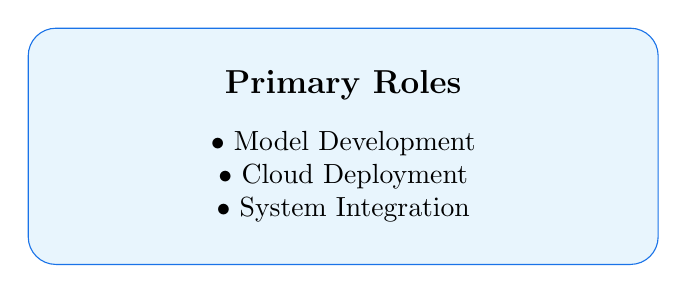
\begin{tikzpicture}
        \node[draw=primaryblue, fill=lightblue, rounded corners=10pt, minimum width=8cm, minimum height=3cm, align=center] {
            \textbf{\large Primary Roles}\\[0.3cm]
            $\bullet$ Model Development\\
            $\bullet$ Cloud Deployment\\
            $\bullet$ System Integration
        };
    \end{tikzpicture}
    
    \vfill
    
    {\large
    \textbf{BTech (Hons.) CSE - Artificial Intelligence}\\
    5th Semester | Group 09\\[0.5cm]
    University Teaching Department (UTD)\\
    CSVTU, Bhilai\\[0.5cm]
    \textbf{December 2025}
    }
    
\end{titlepage}

%========================================
% TABLE OF CONTENTS
%========================================
\tableofcontents
\newpage

%========================================
% SECTION 1: ROLE OVERVIEW
%========================================
\section{Role Overview}

\begin{highlightblock}
\textbf{Assigned Responsibilities:}
\begin{itemize}[leftmargin=*]
    \item[$\triangleright$] \textbf{Model Development} --- YOLOv8 training and optimization
    \item[$\triangleright$] \textbf{Cloud Deployment} --- Hugging Face Spaces deployment
    \item[$\triangleright$] \textbf{System Integration} --- End-to-end pipeline development
\end{itemize}
\end{highlightblock}

\subsection{Contribution Summary}

\begin{table}[H]
    \centering
    \rowcolors{2}{lightgray}{white}
    \begin{tabular}{@{}>{\raggedright}p{4cm}p{8cm}@{}}
        \toprule
        \rowcolor{darkblue}
        \textcolor{white}{\textbf{Area}} & \textcolor{white}{\textbf{Key Contributions}} \\
        \midrule
        Model Development & Trained YOLOv8-Large segmentation model \\
        Training Config & Optimized hyperparameters for 200 epochs \\
        Cloud Deployment & Deployed on Hugging Face Spaces \\
        System Integration & Created unified inference pipeline \\
        \bottomrule
    \end{tabular}
\end{table}

%========================================
% SECTION 2: MODEL DEVELOPMENT
%========================================
\section{Model Development}

\subsection{Model Selection}

Selected \textbf{YOLOv8-Large Segmentation} (yolov8l-seg) for:

\begin{itemize}[leftmargin=*, label=$\checkmark$]
    \item State-of-the-art instance segmentation performance
    \item Balance between accuracy and inference speed
    \item Pre-trained weights for effective transfer learning
    \item Native polygon mask generation support
\end{itemize}

\subsection{Training Configuration}

\begin{table}[H]
    \centering
    \caption{Optimized Training Hyperparameters}
    \rowcolors{2}{lightgray}{white}
    \begin{tabular}{@{}lll@{}}
        \toprule
        \rowcolor{darkblue}
        \textcolor{white}{\textbf{Parameter}} & \textcolor{white}{\textbf{Value}} & \textcolor{white}{\textbf{Rationale}} \\
        \midrule
        Base Model & yolov8l-seg.pt & Large model for accuracy \\
        Epochs & 200 & Sufficient for convergence \\
        Batch Size & 16 & GPU memory optimized \\
        Image Size & 640×640 & Standard YOLO input \\
        Optimizer & AdamW & Better weight decay \\
        Learning Rate & 0.0003 & Tuned for stability \\
        Weight Decay & 0.001 & Regularization \\
        Patience & 50 & Early stopping \\
        \bottomrule
    \end{tabular}
\end{table}

\subsection{Training Implementation}

\begin{lstlisting}[language=Python, caption=YOLOv8 Training Script]
from ultralytics import YOLO

# Load pre-trained model
model = YOLO('yolov8l-seg.pt')

# Train with optimized configuration
results = model.train(
    data='data.yaml',
    epochs=200,
    imgsz=640,
    batch=16,
    optimizer='AdamW',
    lr0=0.0003,
    lrf=0.01,
    weight_decay=0.001,
    patience=50,
    cos_lr=True,
    amp=True,  # Mixed precision
    project='garbage_segmentation',
    name='yolov8l_seg_best'
)
\end{lstlisting}

%========================================
% SECTION 3: CLOUD DEPLOYMENT
%========================================
\section{Cloud Deployment}

\subsection{Platform Selection}

\begin{successblock}
\textbf{Deployed on Hugging Face Spaces}\\[0.3cm]
\url{https://huggingface.co/spaces/Shisodiya/garbage-segmentation}
\end{successblock}

\subsection{Deployment Process}

\begin{enumerate}[leftmargin=*, label=\textbf{Step \arabic*:}]
    \item Created Space with Gradio SDK configuration
    \item Configured Git LFS for 92MB model file
    \item Resolved Gradio/huggingface\_hub version conflicts
    \item Tested and validated live deployment
\end{enumerate}

\subsection{Configuration Files}

\begin{lstlisting}[caption=Hugging Face Space Configuration]
---
title: Garbage Classifier for Waste Management
emoji: trash_can
sdk: gradio
sdk_version: 3.50.2
app_file: app.py
license: mit
---
\end{lstlisting}

%========================================
% SECTION 4: SYSTEM INTEGRATION
%========================================
\section{System Integration}

\subsection{Pipeline Architecture}

\begin{center}
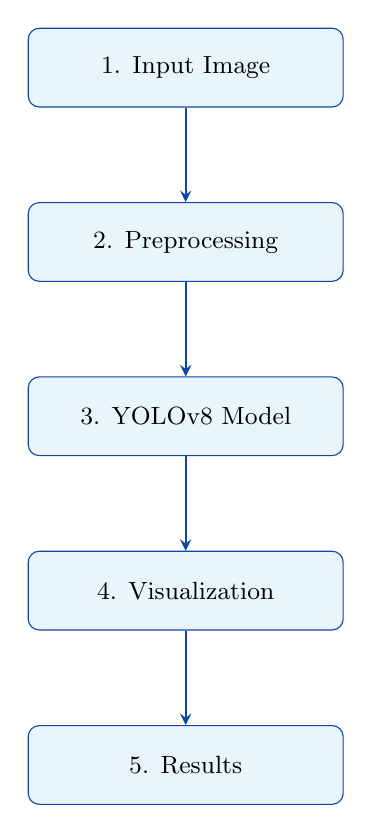
\begin{tikzpicture}[
    node distance=1.2cm,
    box/.style={rectangle, draw=darkblue, fill=lightblue, minimum width=4cm, minimum height=1cm, align=center, rounded corners, font=\small},
    arrow/.style={->, >=stealth, thick, darkblue}
]
    \node[box] (input) {1. Input Image};
    \node[box, below=of input] (preprocess) {2. Preprocessing};
    \node[box, below=of preprocess] (model) {3. YOLOv8 Model};
    \node[box, below=of model] (visualize) {4. Visualization};
    \node[box, below=of visualize] (output) {5. Results};
    
    \draw[arrow] (input) -- (preprocess);
    \draw[arrow] (preprocess) -- (model);
    \draw[arrow] (model) -- (visualize);
    \draw[arrow] (visualize) -- (output);
\end{tikzpicture}
\end{center}

\subsection{Core Integration Code}

\begin{lstlisting}[language=Python, caption=Integrated Inference Pipeline]
class GarbageSegmentor:
    def __init__(self, weights_path='results/best.pt'):
        self.model = YOLO(weights_path)
        self.class_names = [
            'biological', 'cardboard', 'glass',
            'metal', 'paper', 'plastic'
        ]
    
    def segment(self, image):
        results = self.model.predict(image)
        masks = results[0].masks
        boxes = results[0].boxes
        return masks, boxes
    
    def visualize(self, results):
        return results[0].plot()
\end{lstlisting}

%========================================
% SECTION 5: ACHIEVEMENTS
%========================================
\section{Technical Achievements}

\begin{successblock}
\textbf{Key Accomplishments:}
\begin{itemize}[leftmargin=*, label=$\star$]
    \item Successfully trained YOLOv8-Large on 481 images
    \item Achieved high mAP scores for all 6 garbage classes
    \item Deployed production-ready application on cloud
    \item Created efficient, modular inference pipeline
    \item Resolved complex deployment dependencies
\end{itemize}
\end{successblock}

%========================================
% SECTION 6: SKILLS
%========================================
\section{Skills Demonstrated}

\begin{table}[H]
    \centering
    \rowcolors{2}{lightgray}{white}
    \begin{tabular}{@{}ll@{}}
        \toprule
        \rowcolor{darkblue}
        \textcolor{white}{\textbf{Category}} & \textcolor{white}{\textbf{Skills}} \\
        \midrule
        Deep Learning & PyTorch, YOLOv8, Transfer Learning \\
        Computer Vision & Segmentation, Object Detection \\
        Cloud/DevOps & Hugging Face Spaces, Git LFS \\
        Programming & Python, OOP, Modular Design \\
        Tools & Ultralytics, Gradio, OpenCV \\
        \bottomrule
    \end{tabular}
\end{table}

\end{document}
